% В этом документе преамбула

\documentclass[a4paper,12pt]{article}

\usepackage{lscape} % горизонтальный режим
\usepackage{pdflscape}

\usepackage{lipsum} % тестовые тексты

%%% Работа с русским языком
\usepackage{cmap}					% поиск в PDF
\usepackage{mathtext} 				% русские буквы в формулах
\usepackage[T2A]{fontenc}			% кодировка
\usepackage[utf8]{inputenc}			% кодировка исходного текста
\usepackage[english,russian]{babel}	% локализация и переносы
\usepackage{indentfirst}			% чтобы первый абзац в разделе отбивался красной строкой
\frenchspacing						% тонкая настройка пробелов
\usepackage{gensymb}				% символы по типу градусов
\usepackage{algorithm}				% для алгоритмов
\usepackage{algorithmic}			% для алгоритмов

%%% Приведение начертания букв и знаков к русской типографской традиции
\renewcommand{\epsilon}{\ensuremath{\varepsilon}}
\renewcommand{\phi}{\ensuremath{\varphi}}			% буквы "эпсилон"
\renewcommand{\kappa}{\ensuremath{\varkappa}}		% буквы "каппа"
\renewcommand{\le}{\ensuremath{\leqslant}}			% знак меньше или равно
\renewcommand{\leq}{\ensuremath{\leqslant}}			% знак меньше или равно
\renewcommand{\ge}{\ensuremath{\geqslant}}			% знак больше или равно
\renewcommand{\geq}{\ensuremath{\geqslant}}			% знак больше или равно
\renewcommand{\emptyset}{\varnothing}				% знак пустого множества

%%% Дополнительная работа с математикой
\usepackage{amsmath,amsfonts,amssymb,amsthm,mathtools,esint} % AMS
\usepackage{wasysym}
\usepackage{icomma} % "Умная" запятая: $0,2$ --- число, $0, 2$ --- перечисление

%% Номера формул
\mathtoolsset{showonlyrefs=true} % Показывать номера только у тех формул, на которые есть \eqref{} в тексте.

%% Свои команды

% операции, не определённые (или имеющие иные обохначения) в мат. пакетах
\DeclareMathOperator{\sgn}{\mathop{sgn}}				% ф-ия sgn
\renewcommand{\tg}{\mathop{\mathrm{tg}}\nolimits}		% обозначение тангенса

%% Перенос знаков в формулах (по Львовскому)
\newcommand*{\hm}[1]{#1\nobreak\discretionary{}
{\hbox{$\mathsurround=0pt #1$}}{}}

%%% Работа с картинками
\usepackage{graphicx}  				% Для вставки рисунков
\graphicspath{{images/}{images2/}}  % папки с картинками
\setlength\fboxsep{3pt} 			% Отступ рамки \fbox{} от рисунка
\setlength\fboxrule{1pt} 			% Толщина линий рамки \fbox{}
\usepackage{wrapfig} 				% Обтекание рисунков текстом

%%% Работа с таблицами
\usepackage{array,tabularx,tabulary,booktabs} 	% Дополнительная работа с таблицами
\usepackage{longtable}  						% Длинные таблицы
\usepackage{multirow}							% Слияние строк в таблице

%%% Теоремы

\newtheoremstyle{break}% name
	{}%         Space above, empty = `usual value'
	{}%         Space below
	{\itshape}% Body font
	{}%         Indent amount (empty = no indent, \parindent = para indent)
	{\bfseries}% Thm head font
	{.}%        Punctuation after thm head
	{\newline}% Space after thm head: \newline = linebreak
	{}%         Thm head spec
\theoremstyle{break}

% \theoremstyle{plain} % Стиль по умолчанию
\newtheorem{theorem}{Теорема}[section]
\newtheorem{lemma}{Лемма}[section]
\newtheorem{definition}[theorem]{Определение}
\newtheorem{property}{Свойство}
 
\newtheorem{corollary}{Следствие}[theorem]

\newtheoremstyle{example}	% style name
	{2ex}					% above space
	{2ex}					% below space
	{}						% body font
	{}						% indent amount
	{\bf}				% head font
	{.}						% post head punctuation
	{\newline}				% post head punctuation
	{\thmname{#1}\thmnumber{ #2}\thmnote{ (#3)}}						% head spec

\theoremstyle{example}
\newtheorem{exmp}{Пример}[section]
 
\theoremstyle{remark} % "Примечание"
\newtheorem*{nonum}{Решение}
\newtheorem*{evidence}{Доказательство}
\newtheorem*{remark}{Примечание}

%%% Программирование
\usepackage{etoolbox} % логические операторы

%%% Страница
\usepackage{extsizes} % Возможность сделать 14-й шрифт
\usepackage{geometry} % Простой способ задавать поля
	\geometry{top=15mm}
	\geometry{bottom=35mm}
	\geometry{left=10mm}
	\geometry{right=10mm}

%\usepackage{fancyhdr} % Колонтитулы
% 	\pagestyle{fancy}
 	%\renewcommand{\headrulewidth}{0pt}  % Толщина линейки, отчеркивающей верхний колонтитул
% 	\lfoot{Нижний левый}
% 	\rfoot{Нижний правый}
% 	\rhead{Верхний правый}
% 	\chead{Верхний в центре}
% 	\lhead{Верхний левый}
%	\cfoot{Нижний в центре} % По умолчанию здесь номер страницы

\usepackage{setspace} % Интерлиньяж (межстрочные интервалы)
%\onehalfspacing % Интерлиньяж 1.5
%\doublespacing % Интерлиньяж 2
%\singlespacing % Интерлиньяж 1

\usepackage{lastpage} % Узнать, сколько всего страниц в документе.

\usepackage{soulutf8} % Модификаторы начертания

\usepackage{hyperref}
\usepackage[usenames,dvipsnames,svgnames,table,rgb]{xcolor}
\hypersetup{				% Гиперссылки
    unicode=true,           % русские буквы в раздела PDF
    pdftitle={Заголовок},   % Заголовок
    pdfauthor={Автор},      % Автор
    pdfsubject={Тема},      % Тема
    pdfcreator={Создатель}, % Создатель
    pdfproducer={Производитель}, % Производитель
    pdfkeywords={keyword1} {key2} {key3}, % Ключевые слова
    colorlinks=true,       	% false: ссылки в рамках; true: цветные ссылки
    linkcolor=MidnightBlue, % внутренние ссылки
    citecolor=black,        % на библиографию
    filecolor=magenta,      % на файлы
    urlcolor=blue           % на URL
}

\usepackage{csquotes} % Еще инструменты для ссылок

%\usepackage[style=authoryear,maxcitenames=2,backend=biber,sorting=nty]{biblatex}

\usepackage{multicol} % Несколько колонок

%%% Работа с графикой
\usepackage{tikz}
\usetikzlibrary{calc}
\usepackage{tkz-euclide}
\usetikzlibrary{arrows}
\usepackage{pgfplots}
\usepackage{pgfplotstable}

%%% Настройка подписей к плавающим объектам
% \usepackage{floatrow}	% размещение
\usepackage{caption}	% начертание
\captionsetup[figure]{labelfont=bf,textfont=it,font=footnotesize}	% нумерация и надпись курсивом
% для подфигур: заголовок подписи полужирный, текст заголовка обычный
% выравнивание является неровным (т.е. выровненным по левому краю)
% singlelinecheck = off означает, что настройка выравнивания используется, даже если заголовок имеет длину только одну строку.
% если singlelinecheck = on, то заголовок всегда центрируется, когда заголовок состоит только из одной строки.
\captionsetup[subfigure]{labelfont=bf,textfont=normalfont,singlelinecheck=off,justification=raggedright}

%%% Stuff для листинга
\usepackage{listings}
\usepackage{xcolor}

\colorlet{mygray}{black!30}
\colorlet{mygreen}{green!60!blue}
\colorlet{mymauve}{red!60!blue}

\lstset{
	backgroundcolor=\color{gray!10},  
	basicstyle=\ttfamily,
	columns=fullflexible,
	breakatwhitespace=false,      
	breaklines=true,                
	captionpos=b,                    
	commentstyle=\color{mygreen}, 
	extendedchars=true,              
	frame=single,                   
	keepspaces=true,             
	keywordstyle=\color{blue},      
	language=c++,                 
	numbers=none,                
	numbersep=5pt,                   
	numberstyle=\tiny\color{blue}, 
	rulecolor=\color{mygray},        
	showspaces=false,               
	showtabs=false,                 
	stepnumber=5,                  
	stringstyle=\color{mymauve},    
	tabsize=3,                      
	title=\lstname                
}

% для извращённых начертаний
\usepackage{mathrsfs}

\usepackage{makecell}
\setcellgapes{3pt}

% Зачёркивание символов
\usepackage{cancel}

% перечисления с буквами
\usepackage{enumitem}

\DeclareMathOperator{\eq}{\Leftrightarrow}
\DeclareMathOperator\ord{ord}

\title{Специальные разделы алгебры \\ ИДЗ-1 \\ Вариант 54}
\date{16.04.2020}
\author{Почаев Никита Алексеевич, гр. 8381 \\ \href{mailto:pochaev.nik@gmail.com}{pochaev.nik@gmail.com} \\ Преподаватель: Толкачева Елена Алексеевна}

\begin{document}
	
\renewcommand{\figurename}{Рисунок}

\maketitle

\section*{Задача 1.}

\noindent\textbf{\textit{Условие:}}

Функция $f: (\alpha; +\infty) \to (\beta; +\infty)$	задана формулой $f(x) = 2x^2 + 2x + 5$. Найдите наименьшие $\alpha$ и $\beta$, при которых функция $f$ биективна?

\noindent\textbf{\textit{Решение:}}

\begin{center}
	\fbox{%
		\parbox[t][5cm]{16cm}{%
			Отображение $f: A \to B$ называется \textit{биективным} (или биекцией), если оно инъективно и сюръективно одновременно.
			\begin{itemize}
				\item Функция $f: A \to B$ называется \textit{инъективной} (инъекцией), если
				\[\forall a_1, a_2 \in A: a_1 \ne a_2 \Rightarrow f(a_1) \ne f(a_2)\]
				\item Отображение $f: A \to B$ называется \textit{сюръективным} (сюръекцией), если 
				\[\forall b \in B \exists a \in A: f(a) = b\]
			\end{itemize}
	}}\qquad
\end{center}

График функции:
\begin{figure}[H]
	\center{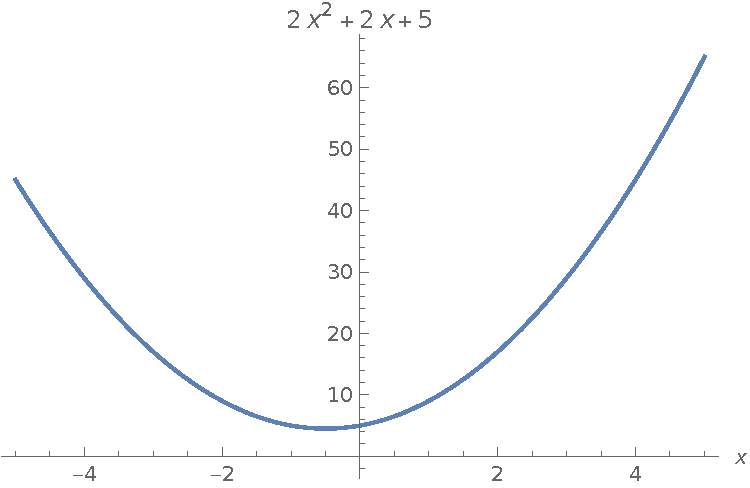
\includegraphics[scale=0.7]{./media/task1.pdf}}
\end{figure}
\noindent Функция $f$ - парабола, найдём координаты её вершины.
\[ y = ax^2 + bx + c, a \ne 0 \Rightarrow \left( \frac{-b}{2a}, -\frac{b^2-4ac}{4a} \right) \]
Таким образом, вершина параболы: $(-0.5, 4.5)$.

Из описанных выше определений следуют следующие условия биективности для заданной функции:
\begin{itemize}
	\item Для сохранения инъективности функция (в данном случае парабола) должна монотонно возрастать/убывать (переводить разные элементы в разные). Если $\alpha < -0.5$, то $\exists a_1, a_2: a_1 \ne a_2 \not\Rightarrow f(a_1) \ne f(a_2)$. Например, для $a_1 = -2, a_2 = 1$ значение функции $f(-2) = f(1) = 9$. Следовательно, $\alpha = -0.5$.
	\item Для сохранения сюръективности каждый элемент из области значений является образом по крайней мере одного элемента из области определения. Значит $\beta = 4.5$, т.к. для $\forall y < 4.5$ прообраз $\emptyset$.
\end{itemize}

\noindent\textbf{Ответ:} $\alpha = -0.5, \beta = 4.5$

\section*{Задача 2.}

\noindent\textbf{\textit{Условие:}}

Является ли функция $f: \{1, \dots, 7\} \to \{1, \dots, 8\}$ заданная таблицей
\[
f =
\begin{pmatrix}
1 & 2 & 3 & 4 & 5 & 6 & 7 \\
5 & 4 & 1 & 7 & 8 & 1 & 2
\end{pmatrix}
\]
инъективной? сюръективной? биективной?

\noindent\textbf{\textit{Решение:}}

\begin{itemize}
	\item Функция \textit{не является инъективной}, т.к. $f(3) = 1$ и $f(6) = 1$, что противоречит определению инъективной ф-ии.
	\item Функция \textit{не является сюръективной}, т.к. не каждый элемент множества $\{1, \dots, 8\}$ является образом хотя бы одного элемента множества $\{1, \dots, 7\}$ - в данном случае это 3 и 6.
	\item Функция \textit{не является биективной}, т.к. данное отображение не инъективно и не сюръективно.
\end{itemize}

\section*{Задача 3.}

\noindent\textbf{\textit{Условие:}}

\begin{enumerate}[label=\alph*)]
	\item Является ли группой $(\mathbb{Z} \textbackslash \{0\}, \cdot)$?
	\item Является ли группой множество всех матриц размера $n \times n$ над $\mathbb{R}$ с определителем 1 операцией сложения?
	\item Является ли группой множество непостоянных линейных функций (многочленов степени 1) с операцией умножения?
\end{enumerate}

\noindent\textbf{\textit{Решение:}}

\begin{center}
	\fbox{%
		\parbox[t][5.5cm]{16cm}{%
			Группа – это множество $G$ с одной замкнутой, ассоциативной, обратимой  алгебраической операцией $*$.
			
			Аксиомы группы:
			\begin{enumerate}
				\item Для любых элементов $a, b, c \in G$ выполняется $(a*b)*c = a*(b*c)$ (аксиома ассоциативности).
				\item Существует элемент $e \in G$ такой, что для любого элемента $a \in G$ выполняется $a*e = e*a = a$ (аксиома нейтрального элемента).
				\item Для $\forall a \in G \exists a^{-1} \in G$ такой, что выполняется $a * a^{-1} = a^{-1} * a = e$ (аксиома обратного элемента).
			\end{enumerate}
	}}\qquad
\end{center}

\begin{enumerate}[label=\alph*)]
	\item Рассмотрим аксиому обратного элемента: пусть $a \in G$, решим уравнение $a \cdot a^{-1} = e$ относительно $a^{-1} \Rightarrow a^{-1} = \frac{e}{a} (e = 1)$, заметим, что множество целых чисел не замкнуто относительно операции деления, которая является обратной умножению, $\Rightarrow a^{-1} \cancel{\in} G$, для $\forall a \ne 1$. Таким образом, $(\mathbb{Z} \textbackslash \{0\}, \cdot)$ \textit{не является} группой.
	\item Данное множество не является замкнутым относительно операции сложения, т.к., например,
	\[
	\begin{pmatrix}
	1 & 0 \\ 0 & 1
	\end{pmatrix}
	+
	\begin{pmatrix}
	1 & 0 \\ 0 & 1
	\end{pmatrix}
	=
	\begin{pmatrix}
	2 & 0 \\ 0 & 2
	\end{pmatrix}
	\]
	У суммируемых матриц определитель равен 1 (они $\in$ мн-ву), а у результирующей 2-м (она $\cancel{\in}$ мн-ву).
	\item Множество непостоянных линейных функций (многочленов степени 1) с операцией умножения не является группой, т.к. не замкнуто относительно операции произведения:
	\[ (ax+b) \cdot (cx+d) = ac\mathbf{x^2} + adx + cbx + bd \]
\end{enumerate}

\section*{Задача 4.}

\noindent\textbf{\textit{Условие:}}

Записать перестановку
\[
\begin{pmatrix}
1 & 2 & 3 & 4 & 5 & 6 & 7 & 8 & 9 & 10 \\
4 & 2 & 1 & 8 & 3 & 9 & 6 & 10 & 7 & 5
\end{pmatrix}
\]
в виде произведения независимых циклов и найти её порядок.

\noindent\textbf{\textit{Решение:}}

\begin{center}
	\fbox{%
		\parbox[t][2.5cm]{16cm}{%
			Циклической перестановкой (циклом) называется перестановка, переводящая $i_1$ в $i_2, i_2$ в $i_3, \dots, i_{k-1}$ в $i_k$ и $i_k$ в $i_1$. Такой цикл кратко записывается в виде $(i_1i_2 \dots i_k)$. Цикл все равно
			откуда начинать. Поэтому, например,
			\[ (i_1i_2 \dots i_k) = (i_2i_3 \dots i_ki_1) \]
	}}\qquad
\end{center}

Данная перестановка в виде цикла представима как:
\[ (1 ~ 4 ~ 8 ~ 10 ~ 5 ~ 3) (2) (6 ~ 9 ~ 7) \]

\begin{center}
	\fbox{%
		\parbox[t][1.8cm]{16cm}{%
			Порядком подстановки называется наименьшая натуральная степень, при возведении в которую получается тождественное преобразование.
			\[ l = \ord u \Leftrightarrow u^l = id \]
	}}\qquad
\end{center}

\[ \ord u = \text{НОК}(6, 1, 3) = 6 \]

\section*{Задача 5.}

\noindent\textbf{\textit{Условие:}}

Найти произведение перестановок: $(2 ~ 8 ~ 3 ~ 6 ~ 5)(4 ~ 7) \cdot (1 ~ 3 ~ 2)(4 ~ 7 ~ 8 ~ 6)$ (ответ в циклической форме).

\noindent\textbf{\textit{Решение:}}

\[
\begin{pmatrix}
1 & 2 & 3 & 4 & 5 & 6 & 7 & 8 \\
1 & 8 & 6 & 7 & 2 & 5 & 4 & 3
\end{pmatrix}
\cdot
\begin{pmatrix}
1 & 2 & 3 & 4 & 5 & 6 & 7 & 8 \\
3 & 1 & 2 & 7 & 5 & 4 & 8 & 6
\end{pmatrix}
=
\begin{pmatrix}
1 & 2 & 3 & 4 & 5 & 6 & 7 & 8 \\
6 & 1 & 8 & 4 & 2 & 7 & 3 & 5
\end{pmatrix}
=
\]
\[
=
(1 ~ 6 ~ 7 ~ 3 ~ 8 ~ 5 ~ 2)(4)
\]

\section*{Задача 6.}

\noindent\textbf{\textit{Условие:}}

Гомоморфизм $\phi: \mathbb{C}^* \to \mathbb{C}^*$ задан формулой $\phi(z) = \frac{z}{|z|}$. Найдите его ядро и образ.

\noindent\textbf{\textit{Решение:}}

\begin{center}
	\fbox{%
		\parbox[t][5.6cm]{16cm}{%
			Отображение $\phi: G_1 \to G_2$ называется \textit{гомоморфизмом групп}, если оно сохраняет результат операции, то есть:
			\[ \forall x, y \in G_1: \phi(x \cdot y) = \phi(x) * \phi(y) \]
			\textit{Ядром гомоморфизма} $\phi$ называется множество:
			\[ Ker \phi = \{ x \in G_1 | \phi(x) = e_2 \} \]
			\textit{Образом гомоморфизма} $\phi$ называется множество:
			\[ Im \phi = \{ y \in G_2 | \exists x \in G_1: \phi(x) = y \} \]
	}}\qquad
\end{center}

Для вычисления ядра решаем уравнение $\underbrace{z}_{\in \mathbb{R}} = \underbrace{|z|}_{\in \mathbb{R}_{>0}} = z$ - положительное вещественное число.
\[ Ker \phi = \mathbb{R}_{>0} \]
Для вычисления образа замечаем, что 
\[ \left| \frac{z}{|z|} \right| = \frac{1}{|z|} \cdot |z| = 1 \]
\[ \Rightarrow Im \phi = \{ z \in \mathbb{C}^* | |z| = 1 \} \]
т.е. образ лежит на окружности радиуса 1 с центром в 0.
\[ Ker \phi = \{ z \in \mathbb{C}^* | \phi(z) = 1 \} \]

\section*{Задача 7.}

\noindent\textbf{\textit{Условие:}}

Пусть $U$ - подгруппа в $GL_3(\mathbb{R})$, состоящая из верхнетреугольных матриц с единицами на главной диагонали, а $H$ - подгруппа в $U$, состоящая из тех матриц, которые отличаются от единичной только на месте $(1, 3)$. Докажите, что $U / H \cong \mathbb{R} \oplus \mathbb{R}$.

\noindent\textbf{\textit{Решение:}}

\begin{center}
	\fbox{%
		\parbox[t][4.6cm]{16cm}{%
			Пусть $(G, \cdot)$ - группа. Непустое подмножество $H$ в $G$ называется подгруппой, если $H$ является группой относительно операции $\cdot$. Иными словами, $H$ является подгруппой, если выполнены следующие
			условия:
			\begin{enumerate}
				\item $H$ замкнуто относительно операции $\cdot$ (т.е $a \cdot b \in H$ для $\forall a, b \in H$);
				\item $H$ замкнуто относительно взятия обратного элемента ($a^{-1} \in H$ для $\forall a \in H$).
			\end{enumerate}
			Рассмотрев любой элемент $a \in H$, получим из свойств (1) и (2), что $a \cdot a^{-1} = e \in H$. Т.е любая подгруппа содержит единицу группы $G$.
	}}\qquad
\end{center}

\[
U = \left\{
\begin{pmatrix}
1 & a & b \\
  & 1 & c \\
0 &   & 1
\end{pmatrix}
\bigg| a, b, c \in \mathbb{R} \right\}
~~~~~~
H = \left\{
\begin{pmatrix}
1 & 0 & a \\
  & 1 & 0 \\
0 &   & 1
\end{pmatrix}
\bigg| a \in \mathbb{R} \right\}
\]

Каждой матрице из $GL_3(\mathbb{R})$\footnote{Полная линейная группа порядка $n$ — это группа обратимых матриц порядка $n$. Роль групповой операции играет обычное умножение матриц.} сопоставляется вектор $(a_{12},a_{23})$ из элементов диагонали выше главной. При перемножении матриц, эти элементы складываются, и получается гомоморфизм в $\mathbb{R} \times \mathbb{R}$, про который также ясно, что он сюръективен. Его ядром будет $H$, поэтому фактогруппа изоморфна $\mathbb{R} \times \mathbb{R}$.

Рассмотрим $\phi: U \to \mathbb{R} \oplus \mathbb{R}$.
\[
\text{Пусть } A = \phi
\begin{pmatrix}
1 & a_1 & b_1 \\
0 & 1 & c_1 \\
0 & 0 & 1
\end{pmatrix}
= (a_1, c_1)
\]
\[
\text{Пусть } B = \phi
\begin{pmatrix}
1 & a_2 & b_2 \\
0 & 1 & c_2 \\
0 & 0 & 1
\end{pmatrix}
= (a_2, c_2)
\]
\[
AB =
\begin{pmatrix}
1 & a_1 & b_1 \\
  & 1 	& c_1 \\
0 &     & 1
\end{pmatrix}
\begin{pmatrix}
1 & a_2 & b_2 \\
  & 1   & c_1 \\
0 &     & 1
\end{pmatrix}
=
\begin{pmatrix}
1 & a_1 + a_2 & b_2 + a_1 & c_2 + b_1 \\
  & 1         & c_1 + c_2 &           \\
  &           & 1         &
\end{pmatrix}
\]
\[ \phi(AB) = (a_1 + a_2, c_1 + c_2) = \phi(A) \phi(B) \Rightarrow \phi - \text{ гомоморфна} \]
$Im \phi = \mathbb{R} \oplus \mathbb{R}$, т.к. $\forall \sigma = (a_1, a_2) \in \mathbb{R} \oplus \mathbb{R}$

\noindent$\exists M \in U, M = \left(\begin{smallmatrix} 1 & a_1 & c \\ & 1 & a_2 \\ 0 & & 1 \end{smallmatrix}\right): \phi(M) = \sigma$

Применяя факт, что $G / Ker \phi \cong Im \phi \Rightarrow U / H \cong \mathbb{R} \oplus \mathbb{R}$.

\section*{Задача 8.}

\noindent\textbf{\textit{Условие:}}

\begin{enumerate}[label=\alph*)]
	\item Лемма Бернсайда.
	\item Приведите пример действия группы на множестве, у которого ровно 1 орбита.
\end{enumerate}

\noindent\textbf{\textit{Решение:}}

\begin{enumerate}[label=\alph*)]
	\item Пусть конечная группа $G$ действует на конечном множестве $X$. Количество орбит действия дается формулой:
	\[ \frac{1}{|G|} \sum_{g \in G} |X_g|, \]
	где $X_g = \{ x \in X | gx = x \}$ - множество неподвижных точек $g$.
	
	\textit{Доказательство:}
	
	Обозначим через $N$ количество таких пар $(g, x)$, что $g(x) = x$. Подсчитаем число $N$ двумя способами.
	
	Вначале просуммируем мощности стабилизаторов всех элементов $x \in X$.  Стабилизаторы точек из орбиты точки $x$, составляющей из $s$ точек, дадут вклад $s|G_x| = (G : G_x)|G_x| = |G|$ (мощность орбиты равна индексу стабилизатора\footnote{$|O_x| = (G : G_x)$ - это следствие из следующего утверждения. Отображение $\phi: y \to \{ g \in G | g(x) = y \}$ сопоставляет каждой точке орбиты $O_x$ класс смежности по стабилизатору $G_x$. Это соответствие взаимно однозначно.}). Т. е. каждая орбита дает вклад $|G|$ в число $N$. Поэтому $N$ равно числу орбит, умноженному на $|G|$.
	
	По-другому число $N$ можно посчитать, суммируя количество неподвижных точек $|X_g|$ по всем $g$. Приравняв два
	полученных выражения и разделив на $|G|$, получаем искомую формулу.
	
	\item Пусть $G = S_n$ и $M = \{1, \dots, n\}$. Имеем естественное действие симметрической группы на множестве $M:$ если $\left(\begin{smallmatrix} 1 & 2 & \dots & n \\ \alpha_1 & \alpha_2 & \dots & \alpha_n \end{smallmatrix}\right) \in S_n$, то $(\alpha, i) \mapsto \alpha(i) = \alpha_i \in M$.
	
	При естественном действии $G = S_n$ на $M = \{ 1, \dots, n \}$ есть всего одна орбита (в этом случае говорят, что $G$ действует транзитивно на $M$). Действительно, для любого $i \in M$ транспозиция $(1 ~ i)$ переводит 1 в $i$, следовательно, $G(1) = M$.
\end{enumerate}

\end{document} 